\documentclass{beamer}
\usepackage[english]{babel}
\usefonttheme{professionalfonts}
\usepackage{geometry}
\usepackage{amsmath}
\usepackage{amsthm}
\usepackage{graphicx}
\usepackage{caption}
\usepackage[utf8]{inputenc}


%%%%%%%% SUB-FIGURE PACKAGE
\usepackage{subcaption}

%%%%%%%% MULTI-COLUMNS PACKAGE
\usepackage{multicol}

%%%%%%%% PERSONAL COMMANDS
\usepackage{amssymb}

%%%% Important sets
\renewcommand{\O}{\mathbb{O}}
\newcommand{\N}{\mathbb{N}}
\newcommand{\Z}{{\mathbb{Z}}}
\newcommand{\Q}{{\mathbb{Q}}}
\newcommand{\R}{{\mathbb{R}}}

%%%% Usual operations
\newcommand{\pow}[2]{#1^{#2}}
\newcommand{\expp}[1]{e^{#1}}
\newcommand{\fst}{\mathrm{fst}}
\newcommand{\snd}{\mathrm{snd}}

%%%% Lambda Calculus
\newcommand{\dneq}{\,\, \# \,\,}
\newcommand{\prm}[1]{\pmb{\mathrm{#1}}}
\renewcommand{\S}{\prm{S}}
\newcommand{\I}{\prm{I}}
\newcommand{\K}{\prm{K}}
\newcommand{\ch}[1]{\ulcorner #1 \urcorner}

%%%% Ordinal Lambda Calculus
\newcommand{\ordAlph}{\Sigma_{\text{Ord}}}
\newcommand{\termOrd}{\text{Term}_\text{Ord}}
\newcommand{\fl}{\mathrm{fl}}
\newcommand{\sk}{\mathrm{sk}}

%% Superscript to the left
% https://latex.org/forum/viewtopic.php?t=455
\usepackage{tensor}
\newcommand{\app}[3]{\tensor*[^{#1}]{\left(#2, #3\right)}{}}

%%%% Make optional parameter
% https://bit.ly/3jVGRwQ
\usepackage{xparse}

%%%% Statistics
\NewDocumentCommand{\E}{o m}{
  \IfNoValueTF{#1}
  {\mathbb{E}\left[#2\right]}
  {\mathbb{E}^{#1}\left[ #2\right]}
}
\NewDocumentCommand{\V}{o m}{
  \IfNoValueTF{#1}
  {\mathrm{Var}\left[#2\right]}
  {\mathrm{Var}^{#1}\left[ #2\right]}
}
\RenewDocumentCommand{\P}{o o m}{
  \IfNoValueTF{#1}
  {\IfNoValueTF{#2}
    {\mathrm{P}\left(#3\right)}
    {\mathrm{P}^{#2}\left(#3\right)}}
  {\IfNoValueTF{#2}
    {\mathrm{P}_{#1}\left(#3\right)}
    {\mathrm{P}_{#1}^{#2} \left(#3\right)}}
}

%%%% Lambda Calculus
\NewDocumentCommand{\cx}{o}{
  \IfNoValueTF{#1}
  {\left[\quad\right]}
  {\left[\, #1 \,\right]}
}

%%%% Create absolute value function
% https://bit.ly/33Rkq6H
\usepackage{mathtools}
\DeclarePairedDelimiter\abs{\lvert}{\rvert}%
\DeclarePairedDelimiter\norm{\lVert}{\rVert}%
\makeatletter
\let\oldabs\abs
\def\abs{\@ifstar{\oldabs}{\oldabs*}}
%
\let\oldnorm\norm
\def\norm{\@ifstar{\oldnorm}{\oldnorm*}}
\makeatother

%%%%%%%% LOGIC TREES
\usepackage{prftree}

%%%%%%%% SPLIT EQUATIONS
% https://bit.ly/33P1OUM
\allowdisplaybreaks

%%%%%%%% FLOAT SPECIFIER
% https://bit.ly/30Wi4BC
\usepackage{float}

%%%%%%%% TO USE SHORT COMMANDS FOR VECTOR LINES
\usepackage{esvect}

%%%%%%%% ENUMERATE LABEL
% https://www.latex-tutorial.com/tutorials/lists/
\usepackage{enumitem}

%%%%%%%% DIFFERENT FONTS FOR MATH
\usepackage{mathrsfs}


%%%%%%%% HYPERREF PACKAGE
\hypersetup{colorlinks=true}
\hypersetup{citecolor=orange}
\hypersetup{urlcolor=orange}

%%%%%%%% DEFINITION AND THEOREM DEFINITIONS
\let\definition\relax
\theoremstyle{definition}
\newtheorem{definition}{Definition}[section]

\let\remark\relax
\theoremstyle{remark}
\newtheorem{remark}{Remark}

\theoremstyle{example}
\newtheorem{question}{Question}

%%%%%%%% BIB-LATEX STUFF
\usepackage[style=authoryear,
            bibstyle=authoryear,
            citestyle=authoryear,
            hyperref=true,
            backend=biber]{biblatex}
\addbibresource{ref.bib} % Bibliography file

%%%%%%%% ICONS FOR CITES
% https://tex.stackexchange.com/questions/68080/beamer-bibliography-icon
\setbeamertemplate{bibliography item}{%
  \ifboolexpr{ test {\ifentrytype{book}} or test {\ifentrytype{mvbook}}
    or test {\ifentrytype{collection}} or test {\ifentrytype{mvcollection}}
    or test {\ifentrytype{reference}} or test {\ifentrytype{mvreference}} }
    {\setbeamertemplate{bibliography item}[book]}
    {\ifentrytype{online}
       {\setbeamertemplate{bibliography item}[online]}
       {\setbeamertemplate{bibliography item}[article]}}
  \usebeamertemplate{bibliography item}}

\defbibenvironment{bibliography}
  {\list{}
     {\settowidth{\labelwidth}{\usebeamertemplate{bibliography item}}
      \setlength{\leftmargin}{\labelwidth}
      \setlength{\labelsep}{\biblabelsep}
      \addtolength{\leftmargin}{\labelsep}
      \setlength{\itemsep}{\bibitemsep}
      \setlength{\parsep}{\bibparsep}}}
  {\endlist}
  {\item}

%%%%%%%% BRACKETS AROUND CITE
% https://bit.ly/3iSxP2u
\makeatletter

\newrobustcmd*{\parentexttrack}[1]{
  \begingroup
  \blx@blxinit
  \blx@setsfcodes
  \blx@bibopenparen#1\blx@bibcloseparen
  \endgroup}

\AtEveryCite{
  \let\parentext=\parentexttrack
  \let\bibopenparen=\bibopenbracket
  \let\bibcloseparen=\bibclosebracket}

\makeatother

%%%%%%%% THEME SLIDES
\usetheme{default}

%%%%%%%% BEAMER STUFF
\setbeamertemplate{footline}[frame number]
\setbeamertemplate{section in toc}[sections numbered]
\setbeamertemplate{subsection in toc}[subsections numbered]
\setbeamertemplate{navigation symbols}{}

% Not enumerate frame breaks
% https://bit.ly/34Rc6TG
\setbeamertemplate{frametitle continuation}[from second][]

%%%%%%%% FRAME TITLES AND SUBTITLES
% https://bit.ly/2FqgWP2
\newif\ifinsection
\newif\ifinsubsection

\let\oldsection\section
\renewcommand{\section}{
  \global\insectiontrue
  \global\insubsectionfalse
  \oldsection}
\let\oldsubsection\subsection
\renewcommand{\subsection}{
  \global\insubsectiontrue
  \oldsubsection}

\newcommand {\aframe}[1] {
  \begin{frame}
    \ifinsection\frametitle{\secname}\fi
    \ifinsubsection\framesubtitle{\subsecname}\fi
  #1
  \end{frame}
}

% Blue line after title
% https://bit.ly/33P6hXm
\setbeamertemplate{frametitle}{%
    \usebeamerfont{frametitle}\insertframetitle\strut%
    \vskip.0\baselineskip%
    \leaders\vrule width 0.85\paperwidth\vskip0.4pt%
    \vskip2pt%
    \usebeamerfont{framesubtitle}\insertframesubtitle
}

% Footnote without symbol
% https://tex.stackexchange.com/questions/30720/footnote-without-a-marker
\newcommand\blfootnote[1]{%
  \begingroup
  \renewcommand\thefootnote{}\footnote{#1}%
  \addtocounter{footnote}{-1}%
  \endgroup
}

%%%%%%%% CENTER OF SLIDE THANK YOU
\usepackage{tikz}

%%%%%%%% CODE RENDERING !!! UNCOMMENT IF NEEDED !!!
% Compile with flag -shell-escape
%\usepackage{minted}


%%%%%%%% START DOCUMENT
\title{System of Advection-Diffusion-Reaction Equations}

\author{Juan Sebasti\'an C\'ardenas-Rodríguez \\
  David Plazas Escudero\\
  \scalebox{0.7}{Mathematical Engineering, Universidad EAFIT}}

\begin{document}

% Plain so is not numbered
\begin{frame}[plain]
  \titlepage
\end{frame}

%%%%%%%%%% SLIDES %%%%%%%%%%%%%%%
\section{Introduction}
\aframe{
Suppose we have two substances $A$ and $B$ that reach chemically on some domain
$\Omega$ to produce $C$:
\[
A+B\rightarrow C.
\]
\begin{itemize}
  \item First-order reaction: rate proportional to the concentrations of $A$
  and $B$.
  \item The formed substance $C$ decays spontaneously with rate proportional to
  its concetration.
  \item We use $u_1$, $u_2$ and $u_3$ to denote the concentrations of $A$, $B$
  and $C$.
\end{itemize}
}


\section{Problem Definition}
\aframe{According to\textcite{langtangen2017}, the formulation of the problem
  is given by the following equations:
  %
  \begin{align*}
    \frac{\partial u_{1}}{\partial t} + w \cdot \nabla u_{1} - \nabla \cdot
    (\epsilon \nabla u_{1}) &= f_{1} - Ku_{1}u_{2} \\
    \frac{\partial u_{2}}{\partial t} + w \cdot \nabla u_{2} - \nabla \cdot
    (\epsilon \nabla u_{2}) &= f_{2} - Ku_{1}u_{2} \\
    \frac{\partial u_{3}}{\partial t} + w \cdot \nabla u_{3} - \nabla \cdot
    (\epsilon \nabla u_{3}) &= f_{3} + Ku_{1}u_{2} - Ku_{3} \\
  \end{align*}
  %
  \begin{overlayarea}{\textwidth}{0.05\textheight}
    \vspace{-1cm}

    \only<2>{We assume that the species $a$, $b$ and $c$ diffuse throughout the
      domain with diffusivity $\epsilon$, are advected with velocity $w$.}

    \only<3->{We assume that the species $a$, $b$ and $c$ diffuse throughout the
      domain with diffusivity $\epsilon$, \textbf{are advected with velocity}
      $\pmb{w}$.}
  \end{overlayarea}
}

\subsection{Navier-Stokes Sub-System}
\aframe{The Navier-Stokes equations for an incompressible fluid for the velocity
  $w$ and a pressure $p$ are given by:
  %
  \begin{align*}
    \frac{\partial w}{\partial t} + w \cdot \nabla w - \nu \nabla^2w +
    \nabla p &= f \\
    \nabla \cdot w &= 0
  \end{align*} \pause
  %
  \begin{itemize}
    \item $\nu$ is the kinematic viscosity.
    \item $f$ is a given source.
  \end{itemize}
}

\section{Weak Formulation}
\subsection{Advection-Diffusion-Reaction Equations}
\aframe{}


\subsection{Navier-Stokes Equations}
\aframe{Let
  %
  \begin{equation*}
    \langle v, w \rangle = \int_{\Omega} vw dx, \quad
    \langle v, w \rangle_{\partial \Omega} = \int_{\partial \Omega} vw ds.
  \end{equation*}
  %
  The Navier-Stokes is solved using a splitting technique proposed
  by\textcite{chorin1968} and\textcite{temam1969}. \vspace{0.5cm} \pause

  First a tentative velocity $w^{*}$ is calculated by ignoring the
  pressure in the momentum, using the following
  \textbf{discrete} variational problem:
  %
  \begin{align*}
    &\Delta t^{-1}\langle w^*_h-w^{n-1}, v\rangle +
      \langle w^{n-1}\cdot\nabla w^{n-1}, v\rangle +
      \langle\nu\nabla w^{n},\nabla v\rangle=\langle f,v\rangle
  \end{align*}
  %
  with $v \in \mathcal{H}_{0}^{1}(\Omega)$.
}

\aframe{On the second step, the tentative velocity $w^{*}$ is used to calculate
  the new pressure $p^{n + 1}$
  \begin{equation*}
    \langle \nabla p^{n},\nabla q\rangle = -\Delta t^{-1}\langle\nabla
      w^*\cdot w^*, q\rangle
  \end{equation*}
  with $q \in \mathcal{H}_{0}^{1}(\Omega)$. \vspace{0.5cm} \pause

  Lastly the corrected velocity $w^{n+1}$ is calculated by
  \begin{equation*}
    \langle w^{n}, v \rangle = \langle w^{*}, v \rangle - \Delta t
    \langle \nabla p^n, v \rangle
  \end{equation*}
}


\section{Results}
\aframe{
Let \[\Lambda=\left\{(x,y)\in\mathbb{R}^2:(x-0.2)^2 + (y-0.2)^2 <
 0.05^2\right\},\] and let \[\Omega=(0,x_f)
 \times(0,y_f) - \Lambda,\] where $y_f=0.41$ and $x_f=2.2$.
 \vspace{0.5cm}
 \begin{figure}
   \centering
   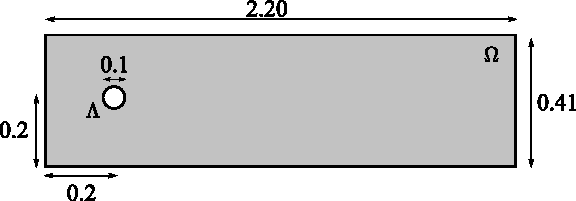
\includegraphics[scale=1]{figs/region.pdf}
 \end{figure}
}

\aframe{
  For the Navier-Stokes part, the boundary conditions are given as
  \begin{align*}
    w(t, 0, y)& = \dfrac{6}{y_f^2}\cdot y(y_f-y),\\
    w(t, x, 0)& = w(t, x, y_f) = w(t, x_f, y) = 0\\
    w(t, x, y)& = 0,\quad \text{over }\partial\Lambda.
  \end{align*}
  The simulation parameters are
  \begin{itemize}
    \item $T=5$.
    \item $N=500$.
    \item $\Delta t=T/N=0.01$.
    \item 
  \end{itemize}
}

%%%%%%%%%%%%%%%%%%%%%%%%%%%%%%%%%
\begin{frame}[allowframebreaks]{References}
  \printbibliography
\end{frame}

\begin{frame}
  \begin{tikzpicture}[overlay, remember picture]
     \node[anchor=center] at (current page.center) {
     \Huge{\emph{Thank you!}}};
\end{tikzpicture}
  \begin{minipage}[t][.8\textheight]{\textwidth}
    \vfill
    \begin{center}
      \begin{multicols}{2}
        \scalebox{0.7}{Juan Sebasti\'an C\'ardenas-Rodríguez} \\
        \scalebox{0.7}{jscardenar@eafit.edu.co} \\

        \columnbreak
        \scalebox{0.7}{David Plazas Escudero} \\
        \scalebox{0.7}{dplazas@eafit.edu.co}
      \end{multicols}
    \end{center}
  \end{minipage}
\end{frame}

\end{document}
